\documentclass{article}

\usepackage[hidelinks]{hyperref}
\usepackage{minted}
\usepackage{xcolor}
\usepackage{tcolorbox}
\usepackage{graphicx}
\usepackage{dirtree}
\usepackage{tabularx}

\graphicspath{{img/}}

\newcommand\tab[1][0.5cm]{\hspace*{#1}}

\definecolor{bg}{HTML}{282828}

\renewcommand{\contentsname}{Table of Contents}

\title{Girls Power Tech 2018 - Google Chrome Malware \& Botnet}
\author{Lilly Chalupowski  \\
	Security Application Developer - Threat Intelligence  \\
	\& 
	Xandria Richman \\
	Cyber Security Analyst - Shift Lead \\
	}

\date{March 3, 2018}

\begin{document}

\begin{titlepage}
  \begin{center}
    
\includegraphics[scale=0.05]{gosecure_logo}\\
    \bigskip
    \LARGE\textbf{Girls Power Tech - Google Chrome Malware \& Botnet}\\
  \end{center}
   \vspace*{\stretch{1.0}}
   \begin{center}
     
\includegraphics[scale=0.3]{aap_logo}
   \end{center}
   \vspace*{\stretch{2.0}}
   \begin{center}
     \small\textbf{Lilly Chalupowski\\
      Security Application Developer - Threat Intelligence\\
      \smallskip
      \&\\
      \smallskip
      Xandria Richman\\
      Cyber Security Analyst - Shift Lead
    }\\
  \end{center}
  \begin{center}
    \large\textbf{May 3, 2018}\\
  \end{center}
\end{titlepage}

\pagebreak

\tableofcontents

\pagebreak

\section{Introduction}
\tab In this handout we will cover the terminology and concepts in the presentation for Chrome extension malware.\\

\section{Disclaimer}\mbox{}\\
\tab The tools and techniques covered in this handout can be dangerous and are being showing for educational purposes only
It is a violation of Federal laws to attempt gaining unauthorized access to information, assets or systems belonging to others, or to exceed authorization on systems for which you have not been granted.
Only use these tools with / on systems you own or have written permission from the owner. We (the speakers) do not assume any responsibility and shall not be held liable for any illegal use of these tools.\\

\pagebreak

\section{Github Repository}
\paragraph{Download Working Files}\mbox{}\\
\begin{tcolorbox}[title=\href{https://github.com/lillypad/chrome-crusader}{chrome-crusader}]
  \usemintedstyle{tango}
  \begin{minted}[fontsize=\small]{bash}
    #!/usr/bin/env bash
    cd ~
    sudo apt-get -qq update
    sudo apt-get -qq -y install git
    git clone https://github.com/lillypad/chrome-crusader.git
    cd ~/chrome-crusader/
  \end{minted}
\end{tcolorbox}
\paragraph{Project Directory Structure}\mbox{}\\
\newline
\tab The project directory structure is as follows:\\
\dirtree{%
  .1 chrome-crusader.
  .2 bin.
  .3 handouts.
  .4 girlspowertech.
  .5 girlspowertech.pdf.
  .3 presentation.
  .4 girlspowertech.
  .5 girlspowertech.pdf.
  .2 configure.sh.
  .2 docs.
  .2 LICENSE.
  .2 Makefile.
  .2 requirements.txt.
  .2 src.
  .3 chrome-optimizer.
  .3 cnc-server.
}
\paragraph{Programming Languages}\mbox{}\\
\newline
\begin{tabularx}{\textwidth}{ X X X }
  \textbullet\ Python & \textbullet\ JavaScript & \textbullet\ JSON\\
\end{tabularx}

\pagebreak

\section{Terminology}
\paragraph{Malware}\mbox{}\\
\begin{tcolorbox}[title=\href{https://en.wikipedia.org/wiki/Malware}{Wikipedia}]
  Software that is intended to damage or disable computers and computer systems.
\end{tcolorbox}
\paragraph{manifest.json}\mbox{}\\
\begin{tcolorbox}[title=\href{https://developer.chrome.com/apps/manifest}{Google Developer Documentation}]
  Every app has a JSON formated manifest.json file, that provides important information.
\end{tcolorbox}
\paragraph{Command \& Control Server}\mbox{}\\
\begin{tcolorbox}[title=\href{https://en.wikipedia.org/wiki/Botnet}{Wikipedia}]
  A computer controlled by an attacker or cybercriminal which is used to send commands to systems compromised by malware and receive stolen data from a target network.
\end{tcolorbox}
\paragraph{Hooking}\mbox{}\\
\begin{tcolorbox}[title=\href{https://en.wikipedia.org/wiki/Hooking}{Wikipedia}]
  In computer programming, hooking covers a range of techniques used to alter or augment the behavior of an operating system, of applications, or of other software components by intercepting function calls or messages or events passed between software components. Code that handles such intercepted function calls, events or messages is called a hook.
\end{tcolorbox}

\pagebreak

\section{Building the Project}
\paragraph{Installing Dependancies}\mbox{}\\
\begin{tcolorbox}[title=install-deps.sh]
  \usemintedstyle{tango}
  \begin{minted}[fontsize=\small]{bash}
    #!/usr/bin/env bash
    sudo apt-get -qq update
    sudo apt-get -qq -y install python \
        python-pip \
        chromium \
        texlive \
        texlive-latex-extra \
        pylint \
        npm \
        nodejs
    sudo npm install -g jshint
  \end{minted}
\end{tcolorbox}
\paragraph{Building}\mbox{}\\
\begin{tcolorbox}[title=build.sh]
  \usemintedstyle{tango}
  \begin{minted}[fontsize=\small]{bash}
    #!/usr/bin/env bash
    make
  \end{minted}
\end{tcolorbox}

\section{Install \& Run}
\paragraph{Installing the Extension}\mbox{}\\
\begin{itemize}
\item Open Google Chrome or Chromium
\item Open Extensions Menu
\item Check Developer mode
\item Load unpacked extension...
\item Browse to the folder src/chrome-optimizer/ and click open
\end{itemize}
\begin{center}
  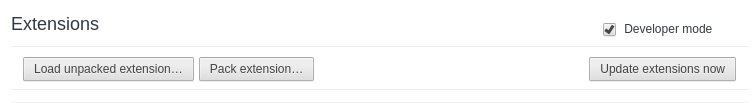
\includegraphics[scale=0.5]{install_extension}
\end{center}
\paragraph{Running the C\&C Sever}\mbox{}\\
\begin{tcolorbox}[title=run-cnc-server.sh]
  \usemintedstyle{tango}
  \begin{minted}[fontsize=\small]{bash}
    #!/usr/bin/env bash
    cd src/cnc-server/scripts/
    ./ccserver.py
  \end{minted}
\end{tcolorbox}
\tab You will now start to see events populate in the sever console.

\pagebreak

\section{Confirm Your Understanding}
\tab Now that you have experienced how this malware works, please try to the best of your ability to answer the following questions. There are questions about your own personal interest in the technology field and these have no right or wrong answer. We really hope you enjoyed the material covered today.

\subsection{Question 1}
\paragraph{Should extensions be trusted even with legitimate company names? Explain why or why not.}\mbox{}\\
\newline
\framebox[\textwidth]{\rule{0pt}{80pt}}

\subsection{Question 2}
\paragraph{If a website requests to install an extension to view the content of the page I would [insert answer]}\mbox{}\\
\newline
\framebox[\textwidth]{\rule{0pt}{80pt}}

\subsection{Question 3}
\paragraph{Is it easy to make malicious extensions? Explain why or why not.}\mbox{}\\
\newline
\framebox[\textwidth]{\rule{0pt}{80pt}}

\pagebreak

\subsection{Question 4}
\paragraph{What does (CnC or C\&C) stand for and why is it important to malware?}\mbox{}\\
\newline
\framebox[\textwidth]{\rule{0pt}{80pt}}

\subsection{Question 5}
\paragraph{What does hooking mean when we are talking about malware?}\mbox{}\\
\newline
\framebox[\textwidth]{\rule{0pt}{80pt}}

\subsection{Question 6}
\paragraph{Would you consider Cyber Security as a profession you are interested in? Explain why or why not.}\mbox{}\\
\newline
\framebox[\textwidth]{\rule{0pt}{80pt}}

\pagebreak

\subsection{Question 7}
\paragraph{Is the technology industry providing enough resources for women at this time? Explain why or why not.}\mbox{}\\
\newline
\framebox[\textwidth]{\rule{0pt}{80pt}}

\subsection{Question 8}
\paragraph{What did you like about the presentation today on Chrome extension malware?}\mbox{}\\
\newline
\framebox[\textwidth]{\rule{0pt}{80pt}}

\subsection{Question 9}
\paragraph{Is there anything we can improve on?}\mbox{}\\
\newline
\framebox[\textwidth]{\rule{0pt}{80pt}}

\pagebreak

\subsection{Question 10}
\paragraph{Tell us a little about why you are interested in technology}\mbox{}\\
\newline
\framebox[\textwidth]{\rule{0pt}{80pt}}

\pagebreak

\section{Summary}
\tab It is important to be aware of what extensions are installed in your browser as malicious extensions can exfiltrate your credentials, cookies, conversations as well as web history. Thank you all for participating, we hope that we have increased your awareness and interest in the Cyber security filed.

\end{document}